\documentclass{article}
\usepackage[automake, acronym, nonumberlist, nopostdot]{glossaries}
\usepackage{cite}
\usepackage{hyperref}
\usepackage{listings}
\usepackage{chngcntr}
\usepackage{graphicx}
\graphicspath{ {./img/} }

\lstset
{
	basicstyle=\small\ttfamily,
	frame=bt,
	numbers=left,
	tabsize=2,
	captionpos=b,
	aboveskip=2em,
	belowskip=2em
}

%%%%%%%%%%%%%%%%%%%%%%%%%%%%%%%%%%%%%%%%%%%%%%%%%%%%%%%%%%%%%%%%%%%%%%%%%%%%%%%%%%%%%%%%%%
%%%%%%%%%%%%%%%%%%%%%%%%%%%%%%%%%%%%%%%%%%%%%%%%%%%%%%%%%%%%%%%%%%%%%%%%%%%%%%%%%%%%%%%%%%
%%%%%
%%%%%	Commands
%%%%%
%%%%%%%%%%%%%%%%%%%%%%%%%%%%%%%%%%%%%%%%%%%%%%%%%%%%%%%%%%%%%%%%%%%%%%%%%%%%%%%%%%%%%%%%%%
%%%%%%%%%%%%%%%%%%%%%%%%%%%%%%%%%%%%%%%%%%%%%%%%%%%%%%%%%%%%%%%%%%%%%%%%%%%%%%%%%%%%%%%%%%

\renewcommand{\lstlistingname}{Code listing}
\renewcommand{\lstlistlistingname}{List of code listings}

%%%%%%%%%%%%%%%%%%%%%%%%%%%%%%%%%%%%%%%%%%%%%%%%%%%%%%%%%%%%%%%%%%%%%%%%%%%%%%%%%%%%%%%%%%
%%%%%%%%%%%%%%%%%%%%%%%%%%%%%%%%%%%%%%%%%%%%%%%%%%%%%%%%%%%%%%%%%%%%%%%%%%%%%%%%%%%%%%%%%%
%%%%%
%%%%%	Create acronyms
%%%%%
%%%%%%%%%%%%%%%%%%%%%%%%%%%%%%%%%%%%%%%%%%%%%%%%%%%%%%%%%%%%%%%%%%%%%%%%%%%%%%%%%%%%%%%%%%
%%%%%%%%%%%%%%%%%%%%%%%%%%%%%%%%%%%%%%%%%%%%%%%%%%%%%%%%%%%%%%%%%%%%%%%%%%%%%%%%%%%%%%%%%%

\newacronym{cil}{CIL}{Common Intermediate Language}
\newacronym{msil}{MSIL}{Microsoft Intermediate Language}
\newacronym{il}{IL}{Intermediate Language}
\newacronym{cli}{CLI}{Common Language Infrastructure}
\newacronym{iso}{ISO}{International Organization for Standardization}
\newacronym{cts}{CTS}{Common Type System}
\newacronym{cls}{CLS}{Common Language Specification}
\newacronym{ves}{VES}{Virtual Execution System}
\newacronym{ast}{AST}{Abstract syntax tree}
\makeglossaries

%%%%%%%%%%%%%%%%%%%%%%%%%%%%%%%%%%%%%%%%%%%%%%%%%%%%%%%%%%%%%%%%%%%%%%%%%%%%%%%%%%%%%%%%%%
%%%%%%%%%%%%%%%%%%%%%%%%%%%%%%%%%%%%%%%%%%%%%%%%%%%%%%%%%%%%%%%%%%%%%%%%%%%%%%%%%%%%%%%%%%
%%%%%
%%%%%	Begin document
%%%%%
%%%%%%%%%%%%%%%%%%%%%%%%%%%%%%%%%%%%%%%%%%%%%%%%%%%%%%%%%%%%%%%%%%%%%%%%%%%%%%%%%%%%%%%%%%
%%%%%%%%%%%%%%%%%%%%%%%%%%%%%%%%%%%%%%%%%%%%%%%%%%%%%%%%%%%%%%%%%%%%%%%%%%%%%%%%%%%%%%%%%%

\begin{document}
\counterwithin{lstlisting}{section}

%%%%%%%%%%%%%%%%%%%%%%%%%%%%%%%%%%%%%%%%%%%%%%%%%%%%%%%%%%%%%%%%%%%%%%%%%%%%%%%%%%%%%%%%%%
%%%%%%%%%%%%%%%%%%%%%%%%%%%%%%%%%%%%%%%%%%%%%%%%%%%%%%%%%%%%%%%%%%%%%%%%%%%%%%%%%%%%%%%%%%
%%%%%
%%%%%	Contents
%%%%%
%%%%%%%%%%%%%%%%%%%%%%%%%%%%%%%%%%%%%%%%%%%%%%%%%%%%%%%%%%%%%%%%%%%%%%%%%%%%%%%%%%%%%%%%%%
%%%%%%%%%%%%%%%%%%%%%%%%%%%%%%%%%%%%%%%%%%%%%%%%%%%%%%%%%%%%%%%%%%%%%%%%%%%%%%%%%%%%%%%%%%

\tableofcontents
\clearpage

%%%%%%%%%%%%%%%%%%%%%%%%%%%%%%%%%%%%%%%%%%%%%%%%%%%%%%%%%%%%%%%%%%%%%%%%%%%%%%%%%%%%%%%%%%
%%%%%%%%%%%%%%%%%%%%%%%%%%%%%%%%%%%%%%%%%%%%%%%%%%%%%%%%%%%%%%%%%%%%%%%%%%%%%%%%%%%%%%%%%%
%%%%%
%%%%%	Acronyms
%%%%%
%%%%%%%%%%%%%%%%%%%%%%%%%%%%%%%%%%%%%%%%%%%%%%%%%%%%%%%%%%%%%%%%%%%%%%%%%%%%%%%%%%%%%%%%%%
%%%%%%%%%%%%%%%%%%%%%%%%%%%%%%%%%%%%%%%%%%%%%%%%%%%%%%%%%%%%%%%%%%%%%%%%%%%%%%%%%%%%%%%%%%

\printglossary[type=\acronymtype]
\clearpage

%%%%%%%%%%%%%%%%%%%%%%%%%%%%%%%%%%%%%%%%%%%%%%%%%%%%%%%%%%%%%%%%%%%%%%%%%%%%%%%%%%%%%%%%%%
%%%%%%%%%%%%%%%%%%%%%%%%%%%%%%%%%%%%%%%%%%%%%%%%%%%%%%%%%%%%%%%%%%%%%%%%%%%%%%%%%%%%%%%%%%
%%%%%
%%%%%	Figures
%%%%%
%%%%%%%%%%%%%%%%%%%%%%%%%%%%%%%%%%%%%%%%%%%%%%%%%%%%%%%%%%%%%%%%%%%%%%%%%%%%%%%%%%%%%%%%%%
%%%%%%%%%%%%%%%%%%%%%%%%%%%%%%%%%%%%%%%%%%%%%%%%%%%%%%%%%%%%%%%%%%%%%%%%%%%%%%%%%%%%%%%%%%

\listoffigures
\clearpage

%%%%%%%%%%%%%%%%%%%%%%%%%%%%%%%%%%%%%%%%%%%%%%%%%%%%%%%%%%%%%%%%%%%%%%%%%%%%%%%%%%%%%%%%%%
%%%%%%%%%%%%%%%%%%%%%%%%%%%%%%%%%%%%%%%%%%%%%%%%%%%%%%%%%%%%%%%%%%%%%%%%%%%%%%%%%%%%%%%%%%
%%%%%
%%%%%	Code listings
%%%%%
%%%%%%%%%%%%%%%%%%%%%%%%%%%%%%%%%%%%%%%%%%%%%%%%%%%%%%%%%%%%%%%%%%%%%%%%%%%%%%%%%%%%%%%%%%
%%%%%%%%%%%%%%%%%%%%%%%%%%%%%%%%%%%%%%%%%%%%%%%%%%%%%%%%%%%%%%%%%%%%%%%%%%%%%%%%%%%%%%%%%%

\lstlistoflistings
\clearpage

%%%%%%%%%%%%%%%%%%%%%%%%%%%%%%%%%%%%%%%%%%%%%%%%%%%%%%%%%%%%%%%%%%%%%%%%%%%%%%%%%%%%%%%%%%
%%%%%%%%%%%%%%%%%%%%%%%%%%%%%%%%%%%%%%%%%%%%%%%%%%%%%%%%%%%%%%%%%%%%%%%%%%%%%%%%%%%%%%%%%%
%%%%%
%%%%%	Introduction
%%%%%
%%%%%%%%%%%%%%%%%%%%%%%%%%%%%%%%%%%%%%%%%%%%%%%%%%%%%%%%%%%%%%%%%%%%%%%%%%%%%%%%%%%%%%%%%%
%%%%%%%%%%%%%%%%%%%%%%%%%%%%%%%%%%%%%%%%%%%%%%%%%%%%%%%%%%%%%%%%%%%%%%%%%%%%%%%%%%%%%%%%%%

\section{Introduction}

\subsection{The \acrlong{cli}}

\textit{The \acrfull{cli}} is a specification developed by \textit{Microsoft} and standardized by \textit{\acrshort{iso}} and \textit{ECMA International} \cite{isoStandard, ecmaStandard}. It describes executable code and an environment that allows numerous programming languages to be executed on various platforms.

The following four main aspects are covered by \textit{the \acrlong{cli}} \cite{ecmaStandard}:
\begin{itemize}
	\item{
		\textbf{\textit{The \acrfull{cts}}} - a type system supporting types and operations found in many programming languages;
	}
	\item{
		\textbf{Metadata} - used for describing and referencing types defined by \textit{the \acrshort{cts}};
	}
	\item{
		\textbf{\textit{The \acrfull{cls}}} - an agreement between language designers and framework designers specifying a subset of \textit{the \acrshort{cts}} and a set of usage conventions;
	}
	\item{
		\textbf{\textit{The \acrfull{ves}}} - responsible for loading and executing programs written for \textit{the \acrshort{cli}}.
	}
\end{itemize}

There are multiple implementations of \textit{the \acrshort{cli}}, for instance: \textit{.NET Framework}, \textit{Shared Source Common Language Infrastructure Implementation}, \textit{.NET Core} and \textit{Mono}.

\subsection{The \acrlong{cil}}

\textit{The \acrfull{cil}} is also known as \textit{the \acrfull{msil}} or simply \textit{the \acrfull{il}} \cite{procsharp7}. It is an object-oriented programming language that is a part of \textit{the \acrshort{cli}}. Each language compatible with \textit{the \acrshort{cli}} is compiled into \textit{the \acrshort{cil}}. Moreover, \textit{the \acrshort{cil}} is the actual language executed by \textit{the \acrshort{ves}}. The language is a reasonable compromise between user-friendly, high-level programming languages and low-level assemblers. Although \textit{the \acrshort{cil}} is human-readable, it is still a stack-based language and writing programs manually is therefore quite difficult.

Technically, \textit{the \acrshort{cil}} is just a set of over 200 instructions and it does not define a syntax for describing \textit{the \acrshort{cli} metadata}. There is another syntax called \textit{ILAsm} - an assembly language for \textit{the \acrshort{cil}} \cite{ecmaStandard}. However, many sources refer to \textit{the \acrshort{cil}} and \textit{ILAsm} interchangeably. Thus, \textit{the \acrshort{cil}} means hereinafter the whole \textit{ILAsm} syntax and \textit{the \acrshort{cil} instruction set} refers to the correct meaning of \textit{the \acrlong{cil}}.

\begin{lstlisting}[
	caption={\textit{Hello world} program},
	label={lst:hello_world}
]
.assembly extern mscorlib {}

.assembly HelloWorld {}

.method static public void main() cil managed
{
	.entrypoint
	.maxstack 1
	ldstr "Hello world!"
	call void [mscorlib]System.Console::WriteLine(string)
	ret
}
\end{lstlisting}

The difference between \textit{ILAsm} and \textit{the \acrshort{cil}} can be easily understood by analysing the \textit{Hello world} program shown in code listing \ref{lst:hello_world}. Lines 1-8 and 12 of the example contain \textit{the \acrshort{cli}} metadata described in \textit{ILasm} syntax whereas lines 9-11 contain actual \textit{\acrshort{cil}} instructions. The detailed meaning of each line can be explained as follows:
\begin{itemize}
	\item{Line 1 informs that an external assembly (\texttt{mscorlib}) should be loaded.}
	\item{Line 3 defines the assembly that should be created as the result of the compiler.}
	\item{Line 5 declares a static public method (\texttt{main}). It also defines that the method contains \textit{\acrshort{cil}} code.}
	\item{Line 6 begins the body of the \texttt{main} method.}
	\item{Line 7 informs that the method should be used as the entry point of the program - it should be called by the compiler as the very first method.}
	\item{Line 8 specifies the maximal size of the evaluation stack associated with the method.}
	\item{Line 9 contains a \texttt{ldstr} instruction. It tells the compiler to put the \textit{Hello world!} string onto the evaluation stack.}
	\item{Line 10 contains a \texttt{call} instruction. It tells the compiler to call the \texttt{WriteLine} method from the \texttt{System.Console} class defined in the \texttt{mscorlib} assembly.}
	\item{Line 11 contains a \texttt{ret} instruction. It tells the compiler to return the result of the method and to transfer the control to the next method on the call stack.}
	\item{Line 12 ends the body of the \texttt{main} method.}
\end{itemize}

\subsection{{TUTAJ ZALOZENIA, CEL PRACY I ZAKONCZENIE WSTEPU}}

\clearpage

%%%%%%%%%%%%%%%%%%%%%%%%%%%%%%%%%%%%%%%%%%%%%%%%%%%%%%%%%%%%%%%%%%%%%%%%%%%%%%%%%%%%%%%%%%
%%%%%%%%%%%%%%%%%%%%%%%%%%%%%%%%%%%%%%%%%%%%%%%%%%%%%%%%%%%%%%%%%%%%%%%%%%%%%%%%%%%%%%%%%%
%%%%%
%%%%%	The CIL instruction set
%%%%%
%%%%%%%%%%%%%%%%%%%%%%%%%%%%%%%%%%%%%%%%%%%%%%%%%%%%%%%%%%%%%%%%%%%%%%%%%%%%%%%%%%%%%%%%%%
%%%%%%%%%%%%%%%%%%%%%%%%%%%%%%%%%%%%%%%%%%%%%%%%%%%%%%%%%%%%%%%%%%%%%%%%%%%%%%%%%%%%%%%%%%

\section{The \acrshort{cil} instruction set}

In order to understand how the \acrshort{cil} instructions work, this section explains the concept of the global state and provides code examples introducing several \acrshort{cil} instructions. As the whole set contains more than 200 instructions, further information on each of them can be found in \cite{ecmaStandard} and \cite{isoStandard}.

\subsection{The global state}

\textit{The \acrshort{cli}} can manage multiple threads of control at the same time. A single thread of control can be thought as a call stack consisting of multiple method states. Although all the threads of control are rather independent, they still can access multiple managed heaps allocated in the shared memory space \cite{ecmaStandard}. This concept is presented in figure \ref{fig:global_state}.

\begin{figure}
	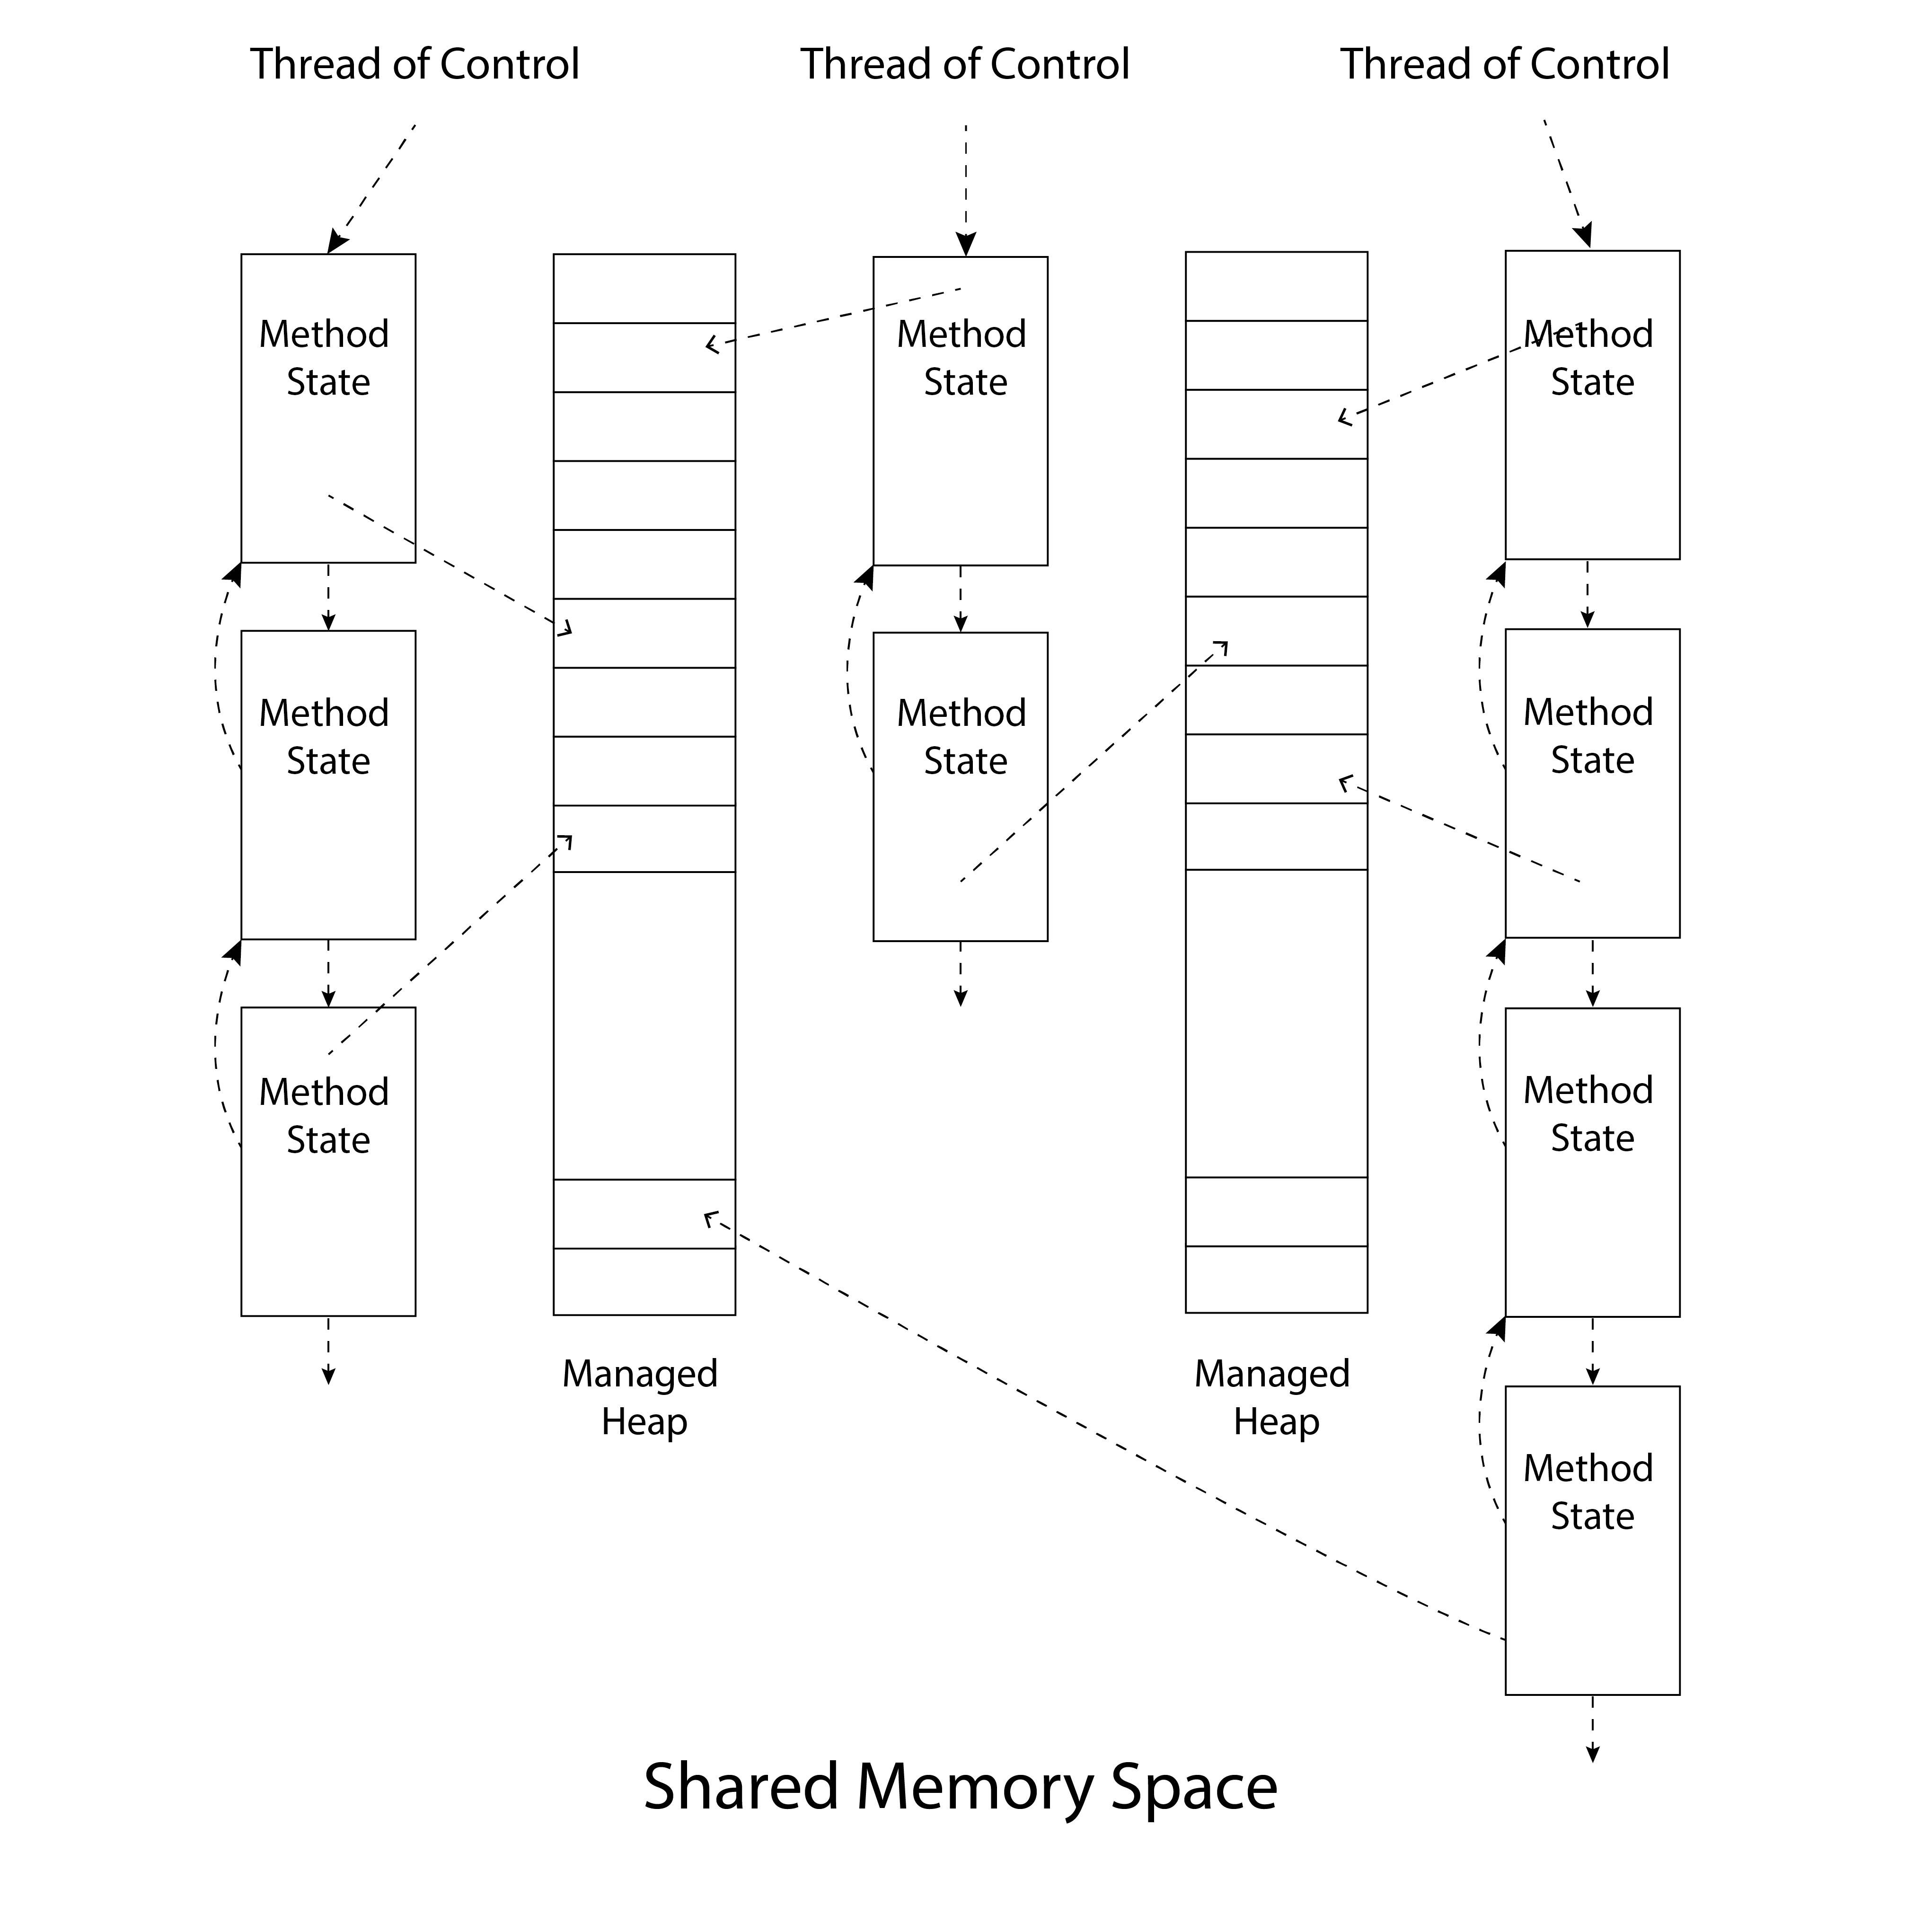
\includegraphics[width=1\textwidth]{global_state.png}
    \centering
    \caption{The global state concept}
    \label{fig:global_state}
\end{figure}

A single method state includes several items required for \textit{the \acrshort{ves}} to execute the method \cite{ecmaStandard}, inter alia:
\begin{itemize}
	\item{an instruction pointer - it determines the next instruction that should be executed within the method;}
	\item{an evaluation stack - it stores evaluation values;}
	\item{a method information handle - it contains read-only method information;}
	\item{a local variable array;}
	\item{an argument array.}
\end{itemize}

Generally, a single instruction can be understood as a description of how to manipulate the corresponding method state - there are only a few exceptions to this rule. Some instructions only require access to the evaluation stack while some do need to change other parts of the global state. To better understand these differences, the examples below present a couple of instructions and describe what effect they have on the global state.

\subsection{The evaluation stack}

As described above, a method state contains an evaluation stack. While a rich set of data types can be represented in memory, only a very limited subset of those types are supported by the \acrshort{cli} on an evaluation stack. This subset consists of the following data types \cite{ecmaStandard}:
\begin{itemize}
	\item{\texttt{int32},}
	\item{\texttt{int64},}
	\item{\texttt{native int},}
	\item{\texttt{F} (a floating-point number),}
	\item{\texttt{O} (an object reference),}
	\item{\texttt{\&} (a managed pointer),}
	\item{\texttt{native unsigned int} (also an unmanaged pointer),}
	\item{a user-defined value type.}
\end{itemize}

\subsection{Stack transformations}

A stack transformation can be thought as a sequence of pop and / or push operations performed on an evaluation stack. The majority of the \acrshort{cil} instructions uses such a sequence to get some values from the corresponding stack or to push some values onto it. In order to describe and visualise the effect of an instruction, the following syntax is used:
\begin{itemize}
	\item{$S$ denotes an evaluation stack;}
	\item{$S \rightarrow S, v_1, v_2, ..., v_n$ denotes a stack transformation which is equivalent to pushing the values $v_1, v_2, ..., v_n$ onto the stack $S$;}
	\item{$S, u_1, u_2, ..., u_n \rightarrow S$ denotes a stack transformation which is equivalent to popping the values $u_1, u_2, ..., u_n$ from the stack $S$;}
	\item{$S, u_1, u_2, ..., u_n \rightarrow S, v_1, v_2, ..., v_m$ denotes a stack transformation which is equivalent to popping values $u_1, u_2, ..., u_n$ from the stack $S$ and then pushing the values $v_1, v_2, ..., v_m$ onto it.}
\end{itemize}

\subsection{The examples}

\subsubsection{\texttt{ldc.i4.0}}

The \texttt{ldc.i4.0} instruction pushes $0$ onto the evaluation stack as \texttt{int32}. The corresponding stack transformation can be presented as follows \cite{ecmaStandard}:
$$
	S \rightarrow S, 0
$$

The program shown in code listing \ref{lst:ldci40} uses the instruction to push $0$ onto the stack and then writes out the top stack value ($0$) using the \texttt{call} instruction.

\begin{lstlisting}[
	caption={Usage of \texttt{ldc.i4.0} instruction},
	label={lst:ldci40}
]
.assembly extern mscorlib {}

.assembly HelloWorld {}

.method static public void main() cil managed
{
	.entrypoint
	.maxstack 1
	ldc.i4.0
	call void [mscorlib]System.Console::WriteLine(int32)
	ret
}
\end{lstlisting}

The \acrshort{cil} provides a number of similar instructions to push other constant values onto the stack: \texttt{ldc.i4.1}, \texttt{ldc.i4.2}, \texttt{ldc.i4.3}, \texttt{ldc.i4.4}, \texttt{ldc.i4.5}, \texttt{ldc.i4.6}, \texttt{ldc.i4.7}, \texttt{ldc.i4.8} and \texttt{ldc.i4.m1} (or \texttt{ldc.i4.M1}) which pushes $-1$ onto the stack.

\subsubsection{{TUTAJ NASTEPNE PRZYKLADY UZYCIA INSTRUKCJI}}

\clearpage

%%%%%%%%%%%%%%%%%%%%%%%%%%%%%%%%%%%%%%%%%%%%%%%%%%%%%%%%%%%%%%%%%%%%%%%%%%%%%%%%%%%%%%%%%%
%%%%%%%%%%%%%%%%%%%%%%%%%%%%%%%%%%%%%%%%%%%%%%%%%%%%%%%%%%%%%%%%%%%%%%%%%%%%%%%%%%%%%%%%%%
%%%%%
%%%%%	The semantics
%%%%%
%%%%%%%%%%%%%%%%%%%%%%%%%%%%%%%%%%%%%%%%%%%%%%%%%%%%%%%%%%%%%%%%%%%%%%%%%%%%%%%%%%%%%%%%%%
%%%%%%%%%%%%%%%%%%%%%%%%%%%%%%%%%%%%%%%%%%%%%%%%%%%%%%%%%%%%%%%%%%%%%%%%%%%%%%%%%%%%%%%%%%

\section{TUTAJ ROZDZIAL O SEMANTYCE}

\clearpage

%%%%%%%%%%%%%%%%%%%%%%%%%%%%%%%%%%%%%%%%%%%%%%%%%%%%%%%%%%%%%%%%%%%%%%%%%%%%%%%%%%%%%%%%%%
%%%%%%%%%%%%%%%%%%%%%%%%%%%%%%%%%%%%%%%%%%%%%%%%%%%%%%%%%%%%%%%%%%%%%%%%%%%%%%%%%%%%%%%%%%
%%%%%
%%%%%	The interpreter
%%%%%
%%%%%%%%%%%%%%%%%%%%%%%%%%%%%%%%%%%%%%%%%%%%%%%%%%%%%%%%%%%%%%%%%%%%%%%%%%%%%%%%%%%%%%%%%%
%%%%%%%%%%%%%%%%%%%%%%%%%%%%%%%%%%%%%%%%%%%%%%%%%%%%%%%%%%%%%%%%%%%%%%%%%%%%%%%%%%%%%%%%%%

\section{The interpreter}

The main part of this thesis is the interpreter which reads a \acrshort{cil} source code and is able to execute it.

TUTAJ KILKA ZDAN / AKAPITOW O TEORII INTERPRETACJI NA PODSTAWIE ZRODEL

\subsection{The lexer and the parser}

TUTAJ KILKA ZDAN O GRAMATYCE, TOKENIZACJI, I PARSOWANIU KODU DO AST

\subsection{Technical background}

In order to focus on the semantics of the \acrshort{cil} and not on data types, the interpreter has been written in \texttt{C\#} which is itself compiled into the \acrshort{cil} so it uses the same type system and the same external assemblies. 

The interpreter is a console application based on the \texttt{.NET Framework 4.7.2} so it can be executed in \texttt{Windows} operating system with the appropriate framework installed. The program can be run with the following command line argument:
\begin{itemize}
	\item{\texttt{--fileName} \texttt{\textit{fileName}} - a path to a text file containing the source code to be interpreted.}
\end{itemize}

The standard input, standard output and standard error streams are redirected to the console in order to allow the interpreted program to interact with the user. For instance, the program shown in code listing \ref{lst:hello_world} calls the \texttt{Console.WriteLine} method to write out the \textit{Hello world!} string to the standard output. The interpreter redirects the output therefore the string appears in the console. However, when an interpreter exception is caught, it is also written to the standard error stream.

\subsection{The actual interpreter}

Before interpreting the provided source code, the application checks if the code is supported by the interpreter. Once a non-supported feature is detected, one of the following exceptions is thrown:
\begin{itemize}
	\item{\texttt{InstructionNotSupportedException},}
	\item{\texttt{FeatureNotSupportedException}.}
\end{itemize}

Each time a new program is interpreted, the interpreter creates 

\clearpage

%%%%%%%%%%%%%%%%%%%%%%%%%%%%%%%%%%%%%%%%%%%%%%%%%%%%%%%%%%%%%%%%%%%%%%%%%%%%%%%%%%%%%%%%%%
%%%%%%%%%%%%%%%%%%%%%%%%%%%%%%%%%%%%%%%%%%%%%%%%%%%%%%%%%%%%%%%%%%%%%%%%%%%%%%%%%%%%%%%%%%
%%%%%
%%%%%	Bibliography
%%%%%
%%%%%%%%%%%%%%%%%%%%%%%%%%%%%%%%%%%%%%%%%%%%%%%%%%%%%%%%%%%%%%%%%%%%%%%%%%%%%%%%%%%%%%%%%%
%%%%%%%%%%%%%%%%%%%%%%%%%%%%%%%%%%%%%%%%%%%%%%%%%%%%%%%%%%%%%%%%%%%%%%%%%%%%%%%%%%%%%%%%%%

\renewcommand{\refname}{Bibliography}

\bibliography{mgr}{}
\bibliographystyle{unsrt}

%%%%%%%%%%%%%%%%%%%%%%%%%%%%%%%%%%%%%%%%%%%%%%%%%%%%%%%%%%%%%%%%%%%%%%%%%%%%%%%%%%%%%%%%%%
%%%%%%%%%%%%%%%%%%%%%%%%%%%%%%%%%%%%%%%%%%%%%%%%%%%%%%%%%%%%%%%%%%%%%%%%%%%%%%%%%%%%%%%%%%
%%%%%
%%%%%	End document
%%%%%
%%%%%%%%%%%%%%%%%%%%%%%%%%%%%%%%%%%%%%%%%%%%%%%%%%%%%%%%%%%%%%%%%%%%%%%%%%%%%%%%%%%%%%%%%%
%%%%%%%%%%%%%%%%%%%%%%%%%%%%%%%%%%%%%%%%%%%%%%%%%%%%%%%%%%%%%%%%%%%%%%%%%%%%%%%%%%%%%%%%%%

\end{document}